%\documentclass[12pt]{article}

\questionheader{ex:s1.3}

%%%%%%%%%%%%%%%%%%
\subsection*{\Conceptual}
%%%%%%%%%%%%%%%%%%

%%%%%%%%%%%%%%%%%%%
\begin{question}\label{prob1.3_signs}
A line in $\mathbb R^2$ has direction $\mathbf d$ and passes through point $\mathbf c$.

Which of the following gives its parametric equation: $\llt x,y\rgt =\mathbf c + t\mathbf d $, or $\llt x,y\rgt =\mathbf c - t\mathbf d $?

\end{question}
\begin{hint}
What, exactly, is $t$?
\end{hint}
\begin{answer}
Both!
\end{answer}
\begin{solution}
Since $t$ can be any real number, these equation describe the same line. They're both valid. For example, the point given by the first parametric 
equation with $t=7$, namely $\mathbf c + 7\mathbf d $, 
is exactly the same as the point given by the second  parametric equation 
with $t=-7$, namely $\mathbf c -(-7)\mathbf d $.
\end{solution}
%%%%%%%%%%%%%%%%%%%

%%%%%%%%%%%%%%%%%%%
\begin{question}
A line in $\mathbb R^2$ has direction $\mathbf d$ and passes through point $\mathbf c$.

Which of the following gives its parametric equation: $\llt x,y\rgt =\mathbf c + t\mathbf d $, or $\llt x,y\rgt =-\mathbf c +t \mathbf d$?

\end{question}
\begin{hint}
What, exactly, is $\mathbf c$?
\end{hint}
\begin{answer}
Generally, only the first.
\end{answer}
\begin{solution}
In contrast to Question~\ref{prob1.3_signs}, the sign on $\mathbf c$ does generally matter. $\mathbf c$ is required to be a point on the line, but except in particular circumstances, there's no reason to believe that 
$-\mathbf c =-\mathbf c +t\mathbf d\big|_{t=0}$ is a point on the line. 
Indeed $-\mathbf c$ is on the line if and only if there is a $t$ with
$\mathbf c + t\mathbf d = -\mathbf c$, i.e. $t\mathbf d = -2\mathbf c$.
That is the case if and only if $\mathbf d$ is parallel to $\mathbf c$.
So, only the first equation is correct in general.
\end{solution}
%%%%%%%%%%%%%%%%%%%

%%%%%%%%%%%%%%%%%%%
%%%%%%%%%%%%%%%%%%%
\begin{question} Two points determine a line. Verify that the equations 

\[\llt x-1,y-9\rgt=t\llt 8,4\rgt\]
and
\[\llt x-9,y-13\rgt=t\llt 1,\tfrac12\rgt\]

describe the same line by finding two different points that lie on both lines.
\end{question}
\begin{hint}
Set $t=0$ in both equation to get two different points with integer coordinates; show that these two points are on both lines.
\end{hint}
\begin{answer}
Since both lines pass through $(1,9)$ and $(9,13)$, the lines are identical.
\end{answer}
\begin{solution}
Here is one answer of many. 

Setting $t=0$ in the first equation shows that
$(1,9)$ is on the first line. To see that $(1,9)$ is also on the second line,
we substitute $x=1$, $y=9$ into the second equation to give
\begin{equation*}
\llt 1-9,9-13\rgt=t\llt 1,\tfrac12\rgt\qquad \text{or}\qquad
\llt -8,-4\rgt=t\llt 1,\tfrac12\rgt
\end{equation*}
This equation is satisfied when $t=-8$. So $(1,9)$ is on both lines.

Setting $t=0$ in the second equation shows that
$(9,13)$ is on the second line. To see that $(9,13)$ is also on the first line,
we substitute $x=9$, $y=13$ into the first equation to give
\begin{equation*}
\llt 9-1,13-9\rgt=t\llt 8,4\rgt\qquad \text{or}\qquad
\llt 8,4\rgt=t\llt 8,4\rgt
\end{equation*}
This equation is satisfied when $t=1$. So $(9,13)$ is on both lines.

Since both lines pass through $(1,9)$ and $(9,13)$, the lines are identical.
\end{solution}
%%%%%%%%%%%%%%%%%%%
\begin{question}
A line in $\mathbb R^2$ has parametric equations
\[\begin{array}{lcl}
x-3&=&9t\\
y-5&=&7t
\end{array}\]
There are many different ways to write the parametric equations of this line. If we rewrite the equations as
\[\begin{array}{lcl}
x-x_0&=&d_xt\\
y-y_0&=&d_yt
\end{array}\]
what are all possible values of $\llt x_0,y_0\rgt$ and $\llt d_x,d_y\rgt$?
\end{question}
\begin{hint}
A line is specified by two things: one point on the line, and a vector parallel to the direction of the line.
\end{hint}
\begin{answer}
$\llt d_x,d_y\rgt$ can be any nonzero scalar multiple of $\llt 9,7\rgt$, and $\llt x_0,y_0\rgt$ can be any point on the line, i.e. any pair that satisfies $7x_0+24=9y_0$.
\end{answer}
\begin{solution}
$\llt d_x,d_y\rgt$ is the direction of the line, so it can be any \textbf{non-zero} scalar multiple of $\llt 9,7\rgt$.

$\llt x_0,y_0\rgt$ can be any point on the line. Describing these is the same as describing the line itself. We're trying to find all 
doubles $\llt x_0,y_0\rgt$  that obey
\begin{align*}
\begin{cases}
x_0-3&=9t\\
y_0-5&=7t
\end{cases}
\end{align*}
for some real number $t$. That is,
\begin{align*}
t=\frac{x_0-3}{9}&=\frac{y_0-5}{7}\\
7(x_0-3)&=9(y_0-5)\\
7x_0+24&=9y_0
\end{align*}

Any of these steps could specify the possible values of $\llt x_0,y_0\rgt$. 
Say, they can be any pair satisfying $7x_0+24=9y_0$.
\end{solution}
%%%%%%%%%%%%%%%%%%%




%%%%%%%%%%%%%%%%%%
\subsection*{\Procedural}
%%%%%%%%%%%%%%%%%%

%%%%%%%%%%%%%%%%%%%%%%%%%%%%%%%%%%%%
\begin{question}
Find the vector parametric, scalar parametric
 and symmetric equations for the line
containing the given point and with the given direction.
\begin{enumerate}[(a)]
\item point $(1,2)$, direction $\llt 3,2\rgt $
\item point $(5,4)$, direction $\llt 2,-1\rgt $
\item point $(-1,3)$, direction $\llt -1,2\rgt $
\end{enumerate}
\end{question}

\begin{hint}
Remember that the parametric equation of a line with direction $\mathbf d$, passing through point $\mathbf c$, is $\llt x,y\rgt =\mathbf c + t\mathbf d $.
\end{hint}

\begin{answer}
(a) $\llt x,y\rgt=\llt 1,2\rgt+t\llt 3,2\rgt $,\ \ \ 
    $x=1+3t,\ y=2+2t$,\ \ \ 
    $\frac{x-1}{3}=\frac{y-2}{2}$

(b) $\llt x,y\rgt=\llt 5,4\rgt+t\llt 2,-1\rgt $,\ \ \ 
    $x=5+2t,\ y=4-t$,\ \ \ 
    $\frac{x-5}{2}=\frac{y-4}{-1}$

(c) $\llt x,y\rgt=\llt -1,3\rgt+t\llt -1,2\rgt $,\ \ \ 
    $x=-1-t,\ y=3+2t$,\ \ \ 
    $\frac{x+1}{-1}=\frac{y-3}{2}$
\end{answer}

\begin{solution}
(a)
The vector parametric equation is $\llt x,y\rgt=\llt 1,2\rgt+t\llt 3,2\rgt $.
The scalar parametric equations are $x=1+3t,\ y=2+2t$.
The symmetric equation is $\frac{x-1}{3}=\frac{y-2}{2}$.

(b)
The vector parametric equation is $\llt x,y\rgt=\llt 5,4\rgt+t\llt 2,-1\rgt $.
The scalar parametric equations are $x=5+2t,\ y=4-t$.
The symmetric equation is $\frac{x-5}{2}=\frac{y-4}{-1}$.

(c)
The vector parametric equation is $\llt x,y\rgt=\llt -1,3\rgt+t\llt -1,2\rgt $.
The scalar parametric equations are $x=-1-t,\ y=3+2t$.
The symmetric equation is $\frac{x+1}{-1}=\frac{y-3}{2}$.
\end{solution}

%%%%%%%%%%%%%%%%%%%%%%%%%%%%%%%%%%%%
\begin{question}
Find the vector parametric, scalar parametric
 and symmetric equations for the line
containing the given point and with the given normal.
\begin{enumerate}[(a)]
\item point $(1,2)$, normal $\llt 3,2\rgt $
\item point $(5,4)$, normal $\llt 2,-1\rgt $
\item point $(-1,3)$, normal $\llt -1,2\rgt $
\end{enumerate}
\end{question}

\begin{hint}
Review Equation~\eref{CLP200}{eqn line} in the CLP-3 text.%1.3.3
\end{hint}

\begin{answer}
(a) $\llt x,y\rgt=\llt 1,2\rgt+t\llt -2,3\rgt $,\ \ \ 
    $x=1-2t,\ y=2+3t$,\ \ \ 
    $\frac{x-1}{-2}=\frac{y-2}{3}$

(b) $\llt x,y\rgt=\llt 5,4\rgt+t\llt 1,2\rgt $,\ \ \ 
    $x=5+t,\ y=4+2t$,\ \ \ 
    $x-5=\frac{y-4}{2}$

(c) $\llt x,y\rgt=\llt -1,3\rgt+t\llt 2,1\rgt $,\ \ \ 
    $x=-1+2t,\ y=3+t$,\ \ \ 
    $\frac{x+1}{2}=y-3$
\end{answer}

\begin{solution}
(a) The vector $\llt -2,3\rgt $ is perpendicular to $\llt 3,2\rgt $ (you can
verify this by taking the dot product of the two vectors) and hence is 
a direction vector for the line.
The vector parametric equation is $\llt x,y\rgt=\llt 1,2\rgt+t\llt -2,3\rgt $.
The scalar parametric equations are $x=1-2t,\ y=2+3t$.
The symmetric equation is $\frac{x-1}{-2}=\frac{y-2}{3}$.

(b) The vector $\llt 1,2\rgt $ is perpendicular to $\llt 2,-1\rgt $ 
 and hence is a direction vector for the line.
The vector parametric equation for the line is 
           $\llt x,y\rgt=\llt 5,4\rgt+t\llt 1,2\rgt $.
The scalar parametric equations are $x=5+t,\ y=4+2t$.
The symmetric equation is $x-5=\frac{y-4}{2}$.

(c) The vector $\llt 2,1\rgt $ is perpendicular to $\llt -1,2\rgt $  
and hence is a direction vector for the line.
The vector parametric equation is $\llt x,y\rgt=\llt -1,3\rgt+t\llt 2,1\rgt $.
The scalar parametric equations are the two component equations $x=-1+2t,\ y=3+t$.
The symmetric equation is $\frac{x+1}{2}=y-3$.
\end{solution}



%%%%%%%%%%%%%%%%%%%%%%%%%%%%%%%%%%%%
\begin{question}
Use a projection to find the distance from the point $(-2,3)$
to the line $3x-4y=-4$.
\end{question}

\begin{hint}
Review Example~\eref{CLP200}{eg nearest point} in the CLP-3 text.%1.3.5
\end{hint}

\begin{answer}
$14/5$
\end{answer}

\begin{solution}
$(0,1)$ is one point on the line $3x-4y=-4$. So $\llt-2-0,3-1\rgt
=\llt-2,2\rgt$ is a vector whose tail is on the line and whose 
head is at $(-2,3)$. $\llt 3,-4\rgt$ is a vector perpendicular to the line,
so $\frac{1}{5}\llt 3,-4\rgt$ is a unit vector perpendicular to the line.
The distance from $(-2,3)$ to the line is the length of the projection 
of $\llt-2,2\rgt$ on $\frac{1}{5}\llt 3,-4\rgt$, which is the magnitude of 
$\frac{1}{5}\llt 3,-4\rgt\cdot\llt -2,2\rgt$. So the distance is $14/5$.
\end{solution}



%%%%%%%%%%%%%%%%%%%%%%%%%%%%%%%%%%%%%
\begin{question}
Let $\va$, $\vb$ and $\vc$ be the vertices of a triangle. By definition, 
a median of a triangle is a straight line that passes through a vertex of 
the triangle and through the midpoint of the opposite side.
\begin{enumerate}[(a)]
\item
 Find the parametric equations of the three medians.
\item
 Do the three medians meet at a common point? If so, which point? 
\end{enumerate}
\end{question}

%\begin{hint}
%\end{hint}

\begin{answer}
(a)
\begin{align*}
\vx(t)&=\va+t\big(\half\vb+\half\vc-\va\big)\\
\vx(s)&=\vb+s\big(\half\va+\half\vc-\vb\big)\\
\vx(u)&=\vc+u\big(\half\va+\half\vb-\vc\big)
\end{align*}

(b)
$\frac{1}{3}(\va+\vb+\vc)$
\end{answer}

\begin{solution}
(a) The midpoint of the side opposite $\va$ is
$\half(\vb+\vc)$. The vector joining $\va$ to that midpoint
is $\half\vb+\half\vc-\va$. The vector parametric equation
of the line through $\va$ and $\half(\vb+\vc)$ is
\begin{equation*}
\vx(t)=\va+t\big(\half\vb+\half\vc-\va\big)
\end{equation*}
Similarly, for the other two medians (but using $s$ and $u$ as
parameters, rather than $t$)
\begin{align*}
\vx(s)&=\vb+s\big(\half\va+\half\vc-\vb\big)\\
\vx(u)&=\vc+u\big(\half\va+\half\vb-\vc\big)
\end{align*}

(b) The three medians meet at a common point if there are
values of $s,t$ and $u$ such that
\begin{alignat*}{3}
\va+t\big(\half\vb+\half\vc-\va\big)
&\ =\ \vb+s\big(\half\va+\half\vc-\vb\big)
&&\ =\ \vc+u\big(\half\va+\half\vb-\vc\big)\\
(1-t)\va+\frac{t}{2}\vb+\frac{t}{2}\vc
&\ =\ \frac{s}{2}\va+(1-s)\vb+\frac{s}{2}\vc
&&\ =\ \frac{u}{2}\va+\frac{u}{2}\vb+(1-u)\vc
\end{alignat*}
Assuming that the triangle has not degenerated to a line segment,
this is the case if and only if the coefficients of $\va,\ \vb$ 
and $\vc$ match
\begin{alignat*}{3}
1-t&=\frac{s}{2}&&=\frac{u}{2}\\
\frac{t}{2}&=1-s&&=\frac{u}{2}\\
\frac{t}{2}&=\frac{s}{2}&&=1-u
\end{alignat*}
or
\begin{equation*}
s=t=u,\  1-t=\frac{t}{2}
\implies
s=t=u=\frac{2}{3}
\end{equation*}
The medians meet at $\frac{1}{3}(\va+\vb+\vc)$.
\end{solution}


%%%%%%%%%%%%%%%%%%%
\begin{question}
Let $C$ be the circle of radius 1 centred at $(2,1)$. Find an equation for the line tangent to $C$ at the point $\left(\frac{5}{2},1+\frac{\sqrt3}{2}\right)$.
\end{question}
\begin{hint}
The radius of the circle will serve as a normal vector to the line.
\end{hint}
\begin{answer}
One way of writing the equation is $x+{\sqrt3}y=4+{\sqrt3}$.
\end{answer}
\begin{solution}
A normal vector to the line is the vector with its tail at the centre of $C$, $(2,1)$, and its head at $\left(\frac{5}{2},1+\frac{\sqrt3}{2}\right)$. 
So, we set $\mathbf{n}=\llt \frac{5}{2},1+\frac{\sqrt3}{2} \rgt-\llt 2,1\rgt = 
\llt \frac12, \frac{\sqrt3}{2}\rgt$.


\begin{center}
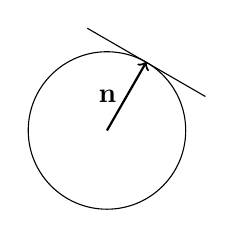
\begin{tikzpicture}
\YEaaxis{.5}{3}{.5}{2}
\draw (2,1) circle (1cm);
%\draw (2,1) node[vertex]{};
\YExcoord{2}{2}
\YEycoord{1}{1}

\draw[thick,->] (2,1)--(2.5,1.87) node[midway, left]{$\mathbf n$};
\draw plot[domain=1.75:3.25](\x,{3.31-\x/1.73});
\end{tikzpicture}
\end{center}

We know one point on the line is $\left(\frac{5}{2},1+\frac{\sqrt3}{2}\right)$, so following Equation~\eref{CLP200}{eqn line}  in the CLP-3 text:
\begin{align*}
n_xx+n_yy&=n_xx_0+n_yy_0\\
\frac12x+\frac{\sqrt3}{2}y&=\frac12\cdot\frac52+\frac{\sqrt3}{2}\cdot\left(1+\frac{\sqrt3}{2}\right)\\
\frac12x+\frac{\sqrt3}{2}y&=2+\frac{\sqrt3}{2}\\
x+{\sqrt3}y&=4+{\sqrt3}\\
\end{align*}
\end{solution}
%%%%%%%%%%%%%%%%%%
%\subsection*{\Application}
%%%%%%%%%%%%%%%%%%
%%%%%%%%%%%%%%%%%%%

%%%%%%%%%%%%%%%%%%%
%%%%%%%%%%%%%%%%%%%